\section{Half-Edge Mesh}
Um ein Traversieren eines Meshes, Abfragen der Nachbarschaftsbeziehungen der einzelnen Meshkomponenten und Operationen wie ,,Subdivisionen'' von Faces (Unterteilung der Faces in kleinere Dreiecke) so einfach wie m\"oglich zu machen, gibt es neben den oben genannten Ans\"atzen noch den Ansatz der Half-Edge Meshes. Ein solches Mesh besteht aus folgenden Komponenten:
\begin{itemize}
	\item eine Liste von Vertices
	\item eine Liste von Half-Edges
	\item eine Liste von Faces.
\end{itemize}

\begin{figure}[h]
	\centering
	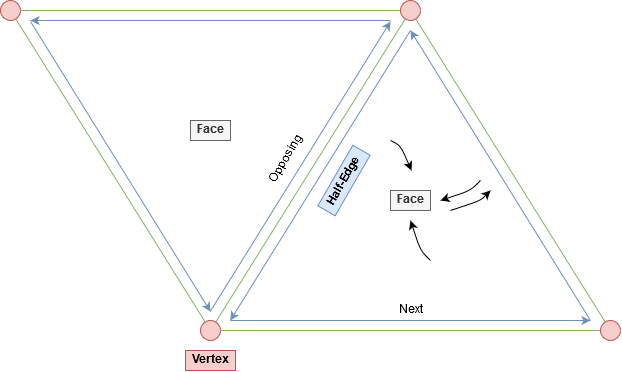
\includegraphics[width=0.7\linewidth]{Images/half-edge-mesh}
	\caption[Half-Edge-Mesh Schematik]{Die Elemente eines Half-Edge-Mesh.}
	\label{fig:half-edge-mesh}
\end{figure}

Im Gegensatz zu den Winged-Edge Meshes modellieren die Half-Edge Meshes eine Kante nicht explizit, sondern als Kombination aus zwei Half-Edges, die in jeweils entgegengesetzte Richtungen auf einen der Endpunkte der Kante zeigen, die Half-Edges sind gegen den Uhrzeigersinn orientiert. Durch die Aufteilung der Kanten kann jede Half-Edge genau einer Face zugeordnet werden und besitzt somit nicht mehr eine Referenz auf den linken und rechten Nachfolger, sondern einen nur noch einen Pointer auf die n\"achste Half-Edge der Face, wie in Abbildung \ref{fig:half-edge-mesh} gezeigt. Zudem Besitzt jede Half-Edge einen Verweis auf die zugeh\"orige Face sowie auf die Gegen\"uberliegende Half-Edge. Ein Verweis auf die Vorherige ist nicht n\"otig, da diese die \"ubern\"achste Kante ist. 

\subsection{Vergleich der Datenstrukturen}
Jede der vorgestellten Datenstrukturen kommt mit Vor- und Nachteilen. Die Entscheidung, welche von diesen verwendet wird, ist vom Use Case der Anwendung abh\"angig. Vergleichen kann man die Datenstrukturen in Sachen Speichernutzung und der Laufzeit von Nachbarschaftsabfragen. Bei der Speichernutzung wird ein allgemeines Mesh mit $n_v$ Vertices betrachtet, bei der Laufzeitanalyse wird zus\"atzlich mit $n_t$ die Anzahl der Dreiecke und mit $m_{ev}$ die Anzahl der Kanten pro Vertex dargestellt.

\begin{table}[ht]
	\caption{Vergleich der Datenstrukturen}
	\centering
		\begin{tabular}{|c|c|c|c|c|}
			\hline 
		& Indexed Mesh & TNS & WEM & HEM \\ 
		\hline 
		Relativer Speicherbedarf & $36 \times n_v  Byte$ & $116 \times n_v  Byte$ & $228 \times n_v  Byte$ & $228 \times n_v  Byte$ \\ 
		\hline 
		\multicolumn{5}{|c|}{Laufzeitanalyse der m\"oglichen Abfragen:} \\ 
		\hline 
		Edge $\rightarrow$ Vertices & N/A  & N/A & $\mathcal{O}(1)$ & $\mathcal{O}(1)$  \\ 
		\hline 
		Edge $\rightarrow$ Faces & N/A & N/A & $\mathcal{O}(1)$ & $\mathcal{O}(1)$ \\ 
		\hline 
		Edge $\rightarrow$ angrenzende Edges & N/A & N/A & $\mathcal{O}(n_{ev})$ & $\mathcal{O}(n_{ev})$ \\ 
		\hline 
		Vertex $\rightarrow$ Edges & $\mathcal{O}(n_t)$ & $\mathcal{O}(n_{ev})$ & $\mathcal{O}(n_{ev})$ & $\mathcal{O}(n_{ev})$ \\ 
		\hline 
		Vertex $\rightarrow$ Faces & $\mathcal{O}(n_t)$ & $\mathcal{O}(n_{ev})$ & $\mathcal{O}(n_{ev})$ & $\mathcal{O}(n_{ev})$ \\ 
		\hline 
		Face $\rightarrow$ Edges & $\mathcal{O}(1)$ & $\mathcal{O}(1)$ & $\mathcal{O}(1)$ & $\mathcal{O}(1)$ \\ 
		\hline 
		Face $\rightarrow$ Vertices & $\mathcal{O}(1)$ & $\mathcal{O}(1)$ & $\mathcal{O}(1)$ & $\mathcal{O}(1)$ \\ 
		\hline 
		Face $\rightarrow$ angrenzende Faces & $\mathcal{O}(n_t)$ & $\mathcal{O}(1)$ & $\mathcal{O}(1)$ & $\mathcal{O}(1)$ \\ 
		\hline 
	\end{tabular} 
	\label{Table:Comp}
\end{table}
Auff\"allig ist, dass der Speicherbedarf mit der Komplexit\"at des Netzes w\"achst, wodurch einzelne Abfragen beschleunigt oder erm\"oglicht werden. Zus\"atzlich f\"allt auf, dass das Winged-Edge Mesh gleich wie das Half-Edge Mesh abschneidet, allerdings bietet das Half-Edge Mesh in der Handhabung gro{\ss}e Erleichterungen, durch eine eindeutige Zuordnung von Half-Edge zu Face.

\subsection{Implementierung der Komponenten}
Die oben beschriebenen Komponenten sind im Folgenden in C\# implementiert, um das Half-Edge Mesh in Unity3D verwenden zu k\"onnen. 

\subsubsection{Klassenstruktur}
Aus den beschriebenen Elementen einer Half-Edge-Netzstruktur ergibt sich das in Abbildung \ref{fig:classdiagramhalfedgemesh} gezeigte Klassendiagramm. Der grundlegende Aufbau der einzelnen Klassen basiert dabei auf dem Plankton-Mesh \cite{Meshmash2017}. Jede Komponente besitzt eine eigene Listenklasse. Allerdings besitzen die einzelnen Komponenten im Plankton-Mesh keine direkte Referenz auf die benachbarten Komponenten, sondern einen Verweis auf den Index der Elemente in der jeweiligen Liste. So hat eine Half-Edge keine weitere Half-Edge als ,,Next'', sondern ein den jeweiligen Index der n\"achsten Kante.

\subsubsection{Die Vertex, HalfEdge und Face Klassen}
Die Klassen \textit{Vertex, HalfEdge} und \textit{Face} sind die Datenmodelle der oben beschriebenen Komponenten. Die Vertex-Klasse besitzt einen \textit{Vector3} Point, der die Position im Raum darstellt, eine \textit{HalfEdge}, die von diesem Punkt aus geht (Im Gegensatz zu \cite{Meshmash2017} wird hier eine Referenz gespeichert.) und der Index des Punktes, um die Arbeit mit dem Unity-Mesh zu erleichtern. Zudem kann ein \textit{PositionChangedEvent} abonniert werden, um Positions\"anderungen im Unity-Mesh direkt zu zeigen.
\\
Eine HalfEdge besitzt die oben erw\"ahnten Eingenschaften: den Punkt von dem sie ausgeht, die anliegende Face, die gegen\"uberliegende und n\"achste HalfEdge sowie den Index der HalfEdge. Wie auch der Index der Vertices, ist dieser Index f\"ur das Unity-Mesh wichtig.
\\
Die Face-Klasse besitzt eine Referenz auf eine anliegende HalfEdge und den Index der Face, diese wieder f\"ur die Arbeit mit dem Unity-Mesh.

\subsubsection{Listenklassen}
Objekte der Klassen \textit{Vertex, HalfEdge, Face} werden jeweils in einer Listenklasse gespeichert. Die Klassen \textit{VertexList, HalfEdgeList, FaceList} implementieren das \textit{IEnumerable}-Interface, um die Iteration \"uber die Elemente zu vereinfachen. Zudem beinhalten diese Klassen die Kernlogiken f\"ur die Komponenten. VertexList bietet die M\"oglichkeit, einen neuen Vertex hinzuzuf\"ugen oder einen zu entfernen, die HalfEdgeList verf\"ugt \"uber eine  \textit{CreateHalfEdge}-Methode, die wie folgt eine HalfEdge anlegt:

\begin{lstlisting}

public HalfEdge CreateHalfEdge(Vertex vertex, Face face, HalfEdge next)
{
	HalfEdge halfEdge = new HalfEdge(vertex, face, next, Count);
	vertex.HalfEdge = halfEdge;
	_halfEdges.Add(halfEdge); // --- _halfEdges ist die zugrunde liegende Liste
	return halfEdge;
}

\end{lstlisting}

Und auch die FaceList besitzt eine Create-Methode, um eine Fl\"ache korrekt anlegen zu k\"onnen. Dabei wird die Referenz der Face auf die HalfEdge gesetzt und umgekehrt. Eine Weitere wichtige Methode ist die \textit{GetFaceCirculator}-Methode, die eine Liste aller HalfEdges, die an einer gegebenen Face anliegen, zur\"uck gibt.

\begin{figure}[t]
	\centering
	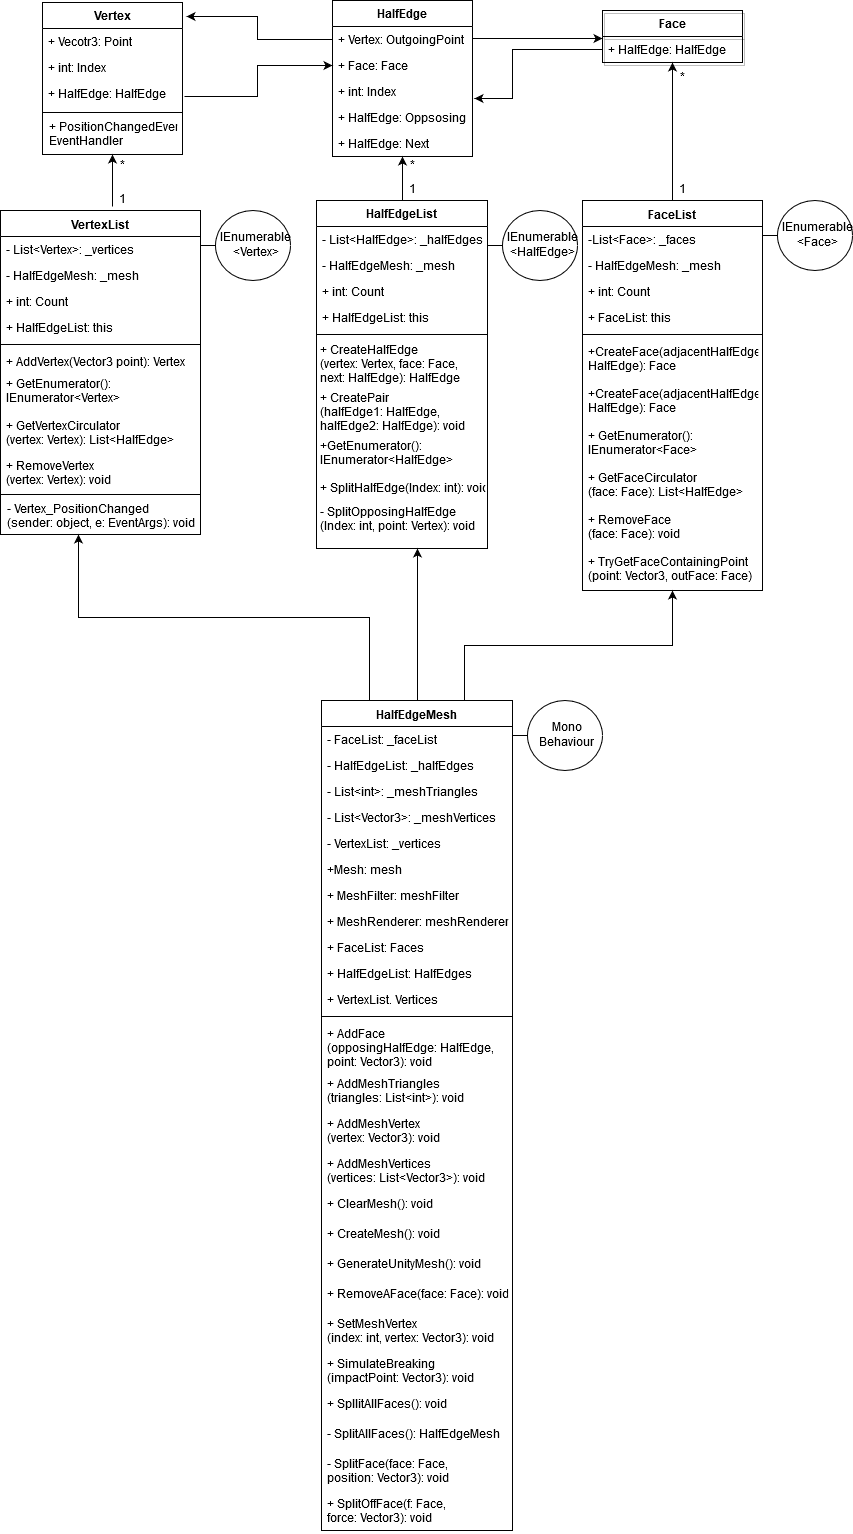
\includegraphics[width=0.7\linewidth]{Images/ClassDiagramHalfEdgeMesh}
	\caption[HalfEdgeMeshUMLDiagramm]{UML-Klassendiagramm des Half-Edge-Mesh Projekts}
	\label{fig:classdiagramhalfedgemesh}
\end{figure}


\subsection{Erstellen eines Half-Edge-Meshes}
Die Oben genannten Listenklassen werden von der \textit{HalfEdgeMesh}-Klasse verwendet, um aus der beschriebenen Half-Edge-Datenstruktur ein von Unity renderbares Mesh zu erstellen. 
\\
Um ein Dreieck, die einfachste m\"ogliche Netzstruktur zu erzeugen, kann die Methode \textit{CreateMesh} verwendet werden. Diese erstellt die drei Eckpunkte des Dreiecks, verbindet zwei mit einer neuen Half-Edge und erzeugt damit ein Face. Die Fl\"ache wird dann verwendet um die fehlenden Kanten mit Referenzen zu erzeugen und anschlie{\ss}end wird die Referenz der ersten Half-Edge auf die zweite gesetzt. Zum Schluss wird \textit{GenerateUnityMesh} aufgerufen um mit den angelegten Daten das UnityMesh zu generieren.
\begin{lstlisting}

public void CreateMesh(Vector3 va, Vector3 vb, Vector3 vc)
{
	Vertex a = Vertices.CreateVertex(va);
	Vertex b = Vertices.CreateVertex(vb);
	Vertex c = Vertices.CreateVertex(vc);

	HalfEdge heA = HalfEdges.CreateHalfEdge(a, null, null);
	Face face = Faces.CreateFace(heA);
	HalfEdge heB = HalfEdges.CreateHalfEdge(b, face, heA);
	HalfEdge heC = HalfEdges.CreateHalfEdge(c, face, heB);
	heA.Next = heC;

	GenerateUnityMesh();
}

\end{lstlisting}
Sollen beim erstellen des Netzes weitere Fl\"achen hinzugef\"ugt werden, ist es m\"oglich diese Methode zu erweitern oder weitere Faces mit \textit{AddFace} hinzuzuf\"ugen.

\subsubsection{GenerateUnityMesh}
Um aus den Daten des Half-Edge-Mesh ein f\"ur Unity brauchbares Mesh zu generieren, m\"ussen folgende Daten aus dem Half-Edge-Mesh entnommen werden: Die Position jedes Punktes, als Liste und ein Array mit der Reihenfolge, wie diese Punkte zu verbinden sind. Die Zusammenstellung dieser Daten passiert mit Hilfe von Linq. Hier der wichtigste Teil der \textit{GenerateUnityMesh}-Methode.
\begin{lstlisting}
	ClearMesh();
	// --- Add vertices
	List<Vertex> vertices = Vertices.Select(p => p.Point).ToList();

	// --- Add triangles
	foreach (Face face in Faces)
	{
		HalfEdge adjacentHalfEdges = Faces.GetFaceCirculator(face).ToList();
		SetMeshTriangles(face.Index, adjacentHalfEdges
		.Select(p => p.OutgoingPoint.Index).ToList(), true);
	}

	AddMeshVertices(vertices);
	CommitMeshTriangles();
\end{lstlisting}
Da das Netz eines komplexen Modells sehr gro{\ss} werden kann, ist es f\"ur die Laufzeit von Vorteil, wenn bei lokalen \"Anderungen nicht das gesamte Netz neu generiert werden muss, wobei jedes Mal \"uber alle Punkte, Kanten und Fl\"achen iteriert werden muss. Stattdessen werden alle Punkte zus\"atzlich in einer Liste gespeichert, die beim bearbeiten des Netzes das UnityMesh aktualisiert. Werden dem Half-Edge-Mesh neue Punkte hinzugef\"ugt, k\"onnen diese mit den Methoden \textit{AddMeshVertex} und \textit{AddMeshVertices} erg\"anzt werden. Am Ende der Methode wird die aktualisierte Liste dem UnityMesh \"ubergeben. 
\\
Auch die Triangles des UnityMeshes werden gecached. Da Manipulationen des Meshes in der Regel bedeuten, dass sich die Triangels relativ zu den drei Punkte einer Face ver\"andern, werden diese in dreier Tuplen in ein Dictionary geschrieben. Der Schl\"ussel ist dabei der Index der Face. Die Indexliste l\"asst sich mit \textit{SetMeshTriangles} bearbeiten. Dabei wird ein Eintrag an der Stelle des Faceindex hinzugef\"ugt, sofern er nicht vorhanden ist oder ver\"andert, falls ein Eintrag existiert. Wichtig ist dies zum Beispiel, wenn eine Face geteilt wird und ein Dreieckseintrag mit zwei von drei Punkten \"ubernommen wird. Als weiteren Parameter kann angegeben werden, ob eine Ver\"anderung Teil einer gr\"o{\ss}eren Transaktion war, um zu vermeiden, dass bei umfangreicheren Operationen, wie der Subdivision aller Faces, f\"ur jeden Methodenaufruf das Dictionary in eine Liste umzuwandeln und das Mesh erneut rendern zu m\"ussen. Wird diese Option verwendet, muss nach Abschluss der Transaktion \textit{CommitMeshTriangles} ausgef\"uhrt werden, um die \"Anderungen ins Mesh zu \"ubernehmen.

\subsubsection{GenerateHalfEdgeMesh}
Andersherum kann es genauso sinnvoll sein, ein bestehendes UnityMesh in ein Half-Edge Mesh umzuwandeln, um die Vorteile dieser nutzen zu k\"onnen. Die Logik dahinter ist in der \textit{HalfEdgeMeshBuilder}-Klasse ausgelagert. Der Builder kann dem HalfEdgeMesh hinzugef\"ugt werden und besitzt eine Referenz auf das HalfEdgeMesh, um dieses bearbeiten zu k\"onnen. Um ein UnityMesh in ein HalfEdgeMesh zu \"uberf\"uhren, kann die \textit{BuildHalfEdgeMeshFromUnityMesh} verwendet werden. Diese Methode f\"ullt die drei Komponentenlisten anhand der Daten aus dem UnityMesh. 
Um dies zu erreichen gelten drei Grunds\"atze:
\begin{enumerate}
	\item F\"ur jeden Punkte gibt es einen Vertex
	\item F\"ur jeden Index gibt es eine HalfEdge, vom Punkt mit dem Index ausgehend
	\item Jeweils drei Indices bilden eine Face.
\end{enumerate}
\begin{lstlisting}
public void BuildHalfEdgeFromUnityMesh(Mesh mesh)
{
	List<Vector3> vertices = mesh.vertices;
	List<int> triangles = mesh.triangles;
	// --- Add vertices to HalfEdgeMesh
	int[] indexChanges = new int[vertices.Length];
	for (int i = 0; i < vertices.Length; i++)
	{
		Vector3 point = vertices[i];
		// --- CreateVertex checks if position is already saved 
		// --- and returns the first matching Vertex
		Vertex vertex = _mesh.Vertices.CreateVertex(point);
		
		// --- Saving the index change
		indexChanges[i] = vertex.Index;
	}
	
	// --- Change Vertex Index to first occurence
	if (indexChanges.Any())
	{
		for (int i = 0; i < triangles.Length; i++)
		{
			// --- change here!
			triangles[i] = indexChanges[triangles[i]];
		}
	}
	
	// --- For every three indices in triangles (= a face) add a face 
	// --- and three halfEdges
	for (int i = 0; i < triangles.Length - 3; i += 3)
	{
		Vertex point1 = _mesh.Vertices[triangles[i]];
		Vertex point2 = _mesh.Vertices[triangles[i + 1]];
		Vertex point3 = _mesh.Vertices[triangles[i + 2]];
		int[] indices = new[] 
		{ point1.Index, point2.Index, point3.Index };
		List<HalfEdges> pairs = _mesh.HalfEdges
		.Where(p => indices.Contains(p.OutgoingPoint.Index)
		&& indices.Contains(p.EndPoint.Index));
	
		HalfEdge halfEdge1 = _mesh.HalfEdges
		.CreateHalfEdge(point1, null, null);
	
		Face face = _mesh.Faces.CreateFace(halfEdge1);
	
		HalfEdge halfEdge2 = _mesh.HalfEdges
		.CreateHalfEdge(point2, face, halfEdge1);
		HalfEdge halfEdge3 = _mesh.HalfEdges
		.CreateHalfEdge(point3, face, halfEdge2);
		halfEdge1.Next = halfEdge3;
	
		foreach (HalfEdge pair in pairs)
		{
			if (pair.OutgoingPoint.Index == halfEdge1.EndPoint.Index 
			&& pair.EndPoint.Index == halfEdge1.OutgoingPoint.Index)
				_mesh.HalfEdges.CreatePair(pair, halfEdge1);
			else if (pair.OutgoingPoint.Index == halfEdge2.EndPoint.Index 
			&& pair.EndPoint.Index == halfEdge2.OutgoingPoint.Index)
				_mesh.HalfEdges.CreatePair(pair, halfEdge2);
			else if (pair.OutgoingPoint.Index == halfEdge3.EndPoint.Index 
			&& pair.EndPoint.Index == halfEdge3.OutgoingPoint.Index)
				_mesh.HalfEdges.CreatePair(pair, halfEdge3);
		}
	}
}
\end{lstlisting}
Beim Erstellen des HalfEdgeMeshes muss beachtet werden, dass beim erzeugen eines Vertex mit \textit{\_mesh.Vertices.CreateVertex(point)} gepr\"uft wird, ob dieser Punkt bereits vorhanden ist, um redundante Daten zu vermeiden und ein zusammenh\"angendes Netz zu garantieren. Wenn in einem UnityMesh allerdings einen Punkt im \textit{vertices}-Array mehrfach vorkommt, verschieben sich nach dieser Stelle alle weiteren Indices. Somit muss zu beginn das UnityMesh ,,bereinigt'' werden. Beim Erstellen der Vertices werden etwaige Index\"anderungen gespeichert und f\"ur alle Indices gepr\"uft. Anschlie{\ss}end werden, wie beim erstellen des UnityMeshes auch, jeweils drei Indices gleichzeitig betrachtet. Zu den Punkten hinter den Indices wird je eine HalfEdge erstellt und zu jeder Triplette wird eine Face erstellt, mit Referenz auf eine der HalfEdges. Zudem m\"ussen alle HalfEdges, die ein Paar mit einer aktuell betrachteten HalfEdge bilden, ermittelt werden. Daf\"ur werden alle HalfEdges gesucht, dessen eingehender und ausgehender Punkt in der Liste der aktuell betrachteten Punkte liegt: 
\begin{lstlisting}
List<HalfEdge> pairs = _mesh.HalfEdges
.Where(p => indices.Contains(p.OutgoingPoint.Index)
&& indices.Contains(p.EndPoint.Index));
\end{lstlisting}